
\begin{frame}{ }
 \begin{center}
  \Large \textbf{How-To: Advanced \ViennaCL}
 \end{center}
\end{frame}


\begin{frame}{How-To: Advanced \ViennaCL}

\begin{block}{What to expect}
  \begin{itemize}
   \item Subvectors and Submatrices
   \item Escaping the Curse of Temporaries
   \item Interface: Eigen
   \item Performance
   \item Summary
  \end{itemize}
\end{block}

\end{frame}



\begin{frame}[fragile]
\frametitle{Subvectors and Submatrices}
 \begin{block}{Important for Many Algorithms}
  \begin{itemize}
   \item LU, Cholesky
   \item QR, SVD
  \end{itemize}
 \end{block}

 \begin{block}{Two sub-types available}
  \begin{itemize}
   \item Range $[a,b)$
   \item Slice $a$:inc:size
  \end{itemize}
 \end{block}

 \begin{block}{Ranges and slices are proxies}
  \begin{itemize}
   \item Read- and writeable
  \end{itemize}
 \end{block}
 
\end{frame}



\begin{frame}[fragile]
\frametitle{Subvectors and Submatrices}

  \begin{block}{Range example}
 \begin{lstlisting}
std::size_t lower_bound = 1;
std::size_t upper_bound = 7;
viennacl::range r(lower_bound, upper_bound);

typedef viennacl::vector<ScalarType> VectorType;
typedef viennacl::matrix<ScalarType> MatrixType;

// v[1:6]
viennacl::vector_range<VCLVectorType> v_sub(v, r);
// M[1:6,1:6]
viennacl::matrix_range<VCLMatrixType> M_sub(M, r, r);
 \end{lstlisting}
 \end{block}

 \vspace{0.45cm}
 
\end{frame}



\begin{frame}[fragile]
\frametitle{Subvectors and Submatrices}

\begin{block}{Slice example}
 \begin{lstlisting}
std::size_t start = 2;
std::size_t stride = 3;
std::size_t size = 5
viennacl::slice s(start, stride, size);

typedef viennacl::vector<ScalarType> VectorType;
typedef viennacl::matrix<ScalarType> MatrixType;

// v[2, 5, 8, 11, 14]
viennacl::vector_slice<VCLVectorType> v_sub(v, r);
// M[2,2], ..., M[2,14], ..., M[14,2], ..., M[14,14]
viennacl::matrix_slice<VCLMatrixType> M_sub(M, r, r);
 \end{lstlisting}
 \end{block}

\end{frame}



\begin{frame}[fragile]
\frametitle{Subvectors and Submatrices}
 \begin{block}{Convenience Functions}
 \begin{lstlisting}
viennacl::vector<ScalarType> v1(4), v2(2);
viennacl::matrix<ScalarType> M1(4,4), M2(2,2);
 
range r(0, 2);
slice s(0, 2, 2);

v2 = project(v1, r);
project(v1, s) = v2;

M2 = project(M1, r, r);
viennacl::copy(M2, project(M1, s, s) );
 \end{lstlisting}
 \end{block}

\end{frame}



\begin{frame}[fragile]
\frametitle{Subvectors and Submatrices}
 \begin{block}{Copy Headaches: Row-Major}
   \begin{center}
     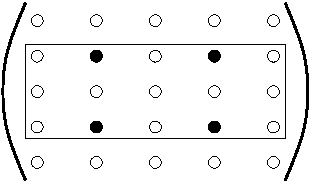
\includegraphics[width=0.35\textwidth]{figs/copy-matrix-row-coarse.pdf} \hspace*{0.5cm}
     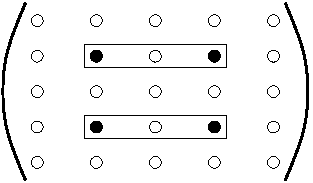
\includegraphics[width=0.35\textwidth]{figs/copy-matrix-row-fine.pdf}
   \end{center}
 \end{block}

 \begin{block}{Copy Headaches: Column-Major}
   \begin{center}
     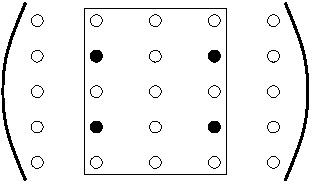
\includegraphics[width=0.35\textwidth]{figs/copy-matrix-col-coarse.pdf} \hspace*{0.5cm}
     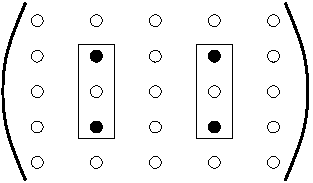
\includegraphics[width=0.35\textwidth]{figs/copy-matrix-col-fine.pdf}
   \end{center}
 \end{block}

\end{frame}





\begin{frame}[fragile]
\frametitle{Escaping the Curse of Temporaries}

 \begin{block}{Simple BLAS Level 1 Operation}
  \begin{itemize}
   \item Consider
  {\black \begin{lstlisting}
 vec1 = vec2 + alpha * vec3 - beta * vec4;
  \end{lstlisting} }

    \item  With naive C++, this is equivalent to
  {\black \begin{lstlisting}
tmp1 <- alpha * vec3
tmp2 <- beta * vec4;
tmp3 <- tmp1 - tmp2;
tmp4 <- vec2 + tmp3;
vec1 <- tmp4;
  \end{lstlisting} }
  \end{itemize}
  
 \end{block}

  \begin{block}{Temporaries Lead to Poor Performance}
    \begin{itemize}
     \item Costly on CPUs, extremely expensive on GPUs
     \item Use expression templates for avoiding temporaries
    \end{itemize}
  \end{block}
  
\vspace*{0.3cm}
\end{frame}




\begin{frame}[fragile]
\frametitle{Escaping the Curse of Temporaries}

 \begin{block}{Vector Addition}
  \begin{lstlisting}
 x = y + z;
  \end{lstlisting}
 \end{block}

  %\pause

 \begin{block}{Naive Operator Overloading}
  \begin{lstlisting}
 vector<T> operator+(vector<T> & v, vector<T> & w);
  \end{lstlisting}

  %\pause

  \begin{itemize}
   \item t $\leftarrow$ y + z, x $\leftarrow$ t
   %\pause
   \item Temporaries are extremely expensive! 
  \end{itemize}
 \end{block}

   %\pause



\end{frame}



\begin{frame}[fragile]
\frametitle{Escaping the Curse of Temporaries}
 \begin{block}{Expression Templates}
  \begin{lstlisting}
 vector_expr<vector<T>, op_plus, vector<T> >
 operator+(vector<T> & v, vector<T> & w) { ... }

 vector::operator=(vector_expr<...> const & e) {
   viennacl::linalg::avbv(*this, 1,e.lhs(), 1,e.rhs());
 }
  \end{lstlisting}
  \vspace*{0.5cm}

 \end{block}

%  \begin{block}{\texttt{vector\_expression} does not compute anything}
%    \begin{itemize}
%     \item Represents the expression only
%    \end{itemize}
%  \end{block}

  \begin{block}{Allows to Avoid a Significant Amount of Temporaries}
    \begin{itemize}
     \item Covers most frequent cases
     \item Influence on compilation times moderate
    \end{itemize}
  \end{block}
\end{frame}



\begin{frame}[fragile]
\frametitle{Escaping the Curse of Temporaries}
  \begin{block}{Expression templates have their limitations}
  \begin{lstlisting}
viennacl::vector<NumericType> v;
viennacl::matrix<NumericType> M;

v = viennacl::linalg::prod(M, v);
  \end{lstlisting}
  
    \begin{itemize}
     \item Temporary object is required here!
     \item ViennaCL detects such cases and takes care of it
    \end{itemize}
 \end{block}

\end{frame}



\begin{frame}{Interface: Eigen}
\begin{block}{Data transfer}
 \begin{itemize}
  \item Like transfer from and to std container
  \item Using provided copy functions
 \end{itemize}
\end{block}

\begin{block}{Interface compatibility}
 \begin{itemize}
  \item ViennaCL algorithms work with Eigen
  \item e.g.: iterative solver
 \end{itemize}
\end{block}
\end{frame}



\begin{frame}[fragile]
\frametitle{Interface: Eigen}
\begin{block}{Data transfer: vectors}
  \begin{lstlisting}
#define VIENNACL_HAVE_EIGEN
 
Eigen::VectorXd eigen_vector(dim);
 
// fill Eigen objects in a very sophisticated way with numbers here
 
viennacl::vector<double> viennacl_vector(dim);
 
// copy data from Eigen objects to ViennaCL objects
viennacl::copy(eigen_vector, viennacl_vector);
 
// do some heavy linear algebra with ViennaCL here 
 
// copy back to Eigen:
viennacl::copy(viennacl_vector, eigen_vector);
  \end{lstlisting} 
\end{block}

\end{frame}



\begin{frame}[fragile]
\frametitle{Interface: Eigen}
\begin{block}{Data transfer: dense matrix}
  \begin{lstlisting}
#define VIENNACL_HAVE_EIGEN
 
Eigen::MatrixXd eigen_densematrix(dim, dim);
 
// fill Eigen objects in a very sophisticated way with numbers here
 
viennacl::matrix<double> viennacl_densematrix(dim, dim);
 
// copy data from Eigen objects to ViennaCL objects
viennacl::copy(eigen_densematrix,viennacl_densematrix);
 
// do some heavy linear algebra with ViennaCL here 
 
// copy back to Eigen:
viennacl::copy(viennacl_densematrix, eigen_densematrix);
  \end{lstlisting} 
\end{block}

\end{frame}



\begin{frame}[fragile]
\frametitle{Interface: Eigen}
\begin{block}{Data transfer: sparse matrix}
  \begin{lstlisting}
#define VIENNACL_HAVE_EIGEN
 
Eigen::SparseMatrix<double, Eigen::RowMajor> eigen_sparsematrix(dim, dim);
 
// fill Eigen objects in a very sophisticated way with numbers here
 
viennacl::compressed_matrix<double> viennacl_sparsematrix(dim, dim);
 
// copy data from Eigen objects to ViennaCL objects
viennacl::copy(eigen_sparsematrix, viennacl_sparsematrix);
 
// do some heavy linear algebra with ViennaCL here 
 
// copy back to Eigen:
viennacl::copy(viennacl_sparsematrix, eigen_sparsematrix);
  \end{lstlisting} 
\end{block}

\end{frame}



\begin{frame}[fragile]
\frametitle{Interface: Eigen}
\begin{block}{Interface Compatibility: iterative solver}
  \begin{lstlisting}
#define VIENNACL_HAVE_EIGEN
using namespace viennacl::linalg;
 
Eigen::SparseMatrix<double, Eigen::RowMajor>
    matrix(dim, dim);
Eigen::VectorXd rhs(dim);
Eigen::VectorXd result(dim);
// fill eigen_matrix and eigen_rhs here
 
// Solve system using CG from ViennaCL
result = solve(matrix, rhs, cg_tag());
 
// Solve system using BiCGStab from ViennaCL
result = solve(matrix, rhs, bicgstab_tag());
 
// Solve system using GMRES from ViennaCL
result = solve(matrix, rhs, gmres_tag());
  \end{lstlisting} 
\end{block}

\end{frame}






%%%%%%%

\begin{frame}[fragile]
\frametitle{Performance}
 \begin{block}{Granularity of Operations}
  \begin{itemize}
   \item Solving linear systems
   \begin{lstlisting}
viennacl::matrix<double> mat(N, N);
viennacl::vector<double> rhs(N);

for (size_t i=0; i<1000; ++i)
{
   viennacl::vector<double> result 
     = solve(mat, rhs, bicgstab_tag());
   /* process result */
}
   \end{lstlisting}
  \end{itemize}
 \end{block}

 \begin{block}{Why Is There No Speed-Up?}
   \begin{itemize}
    \item 
   \end{itemize}
 \end{block}

\end{frame}


\begin{frame}[fragile]
\frametitle{Performance}
 \begin{block}{Granularity of Operations}
  \begin{itemize}
   \item Solving linear systems
   \begin{lstlisting}
viennacl::matrix<double> mat(N, N);
viennacl::vector<double> rhs(N);

for (size_t i=0; i<1000; ++i)
{
   viennacl::vector<double> result 
     = solve(mat, rhs, bicgstab_tag());
   /* process result */
}
   \end{lstlisting}
  \end{itemize}
 \end{block}

 \begin{block}{Why Is There No Speed-Up?}
   \begin{itemize}
    \item $N = 3$
   \end{itemize}
 \end{block}

\end{frame}


\begin{frame}[fragile]
\frametitle{Performance}

Lets take a look

\end{frame}



\begin{frame}[fragile]
\frametitle{Performance}
 \begin{block}{Sample Operation}
  \begin{itemize}
   \item $v_1 \leftarrow v_2$
  \end{itemize}

   \begin{center}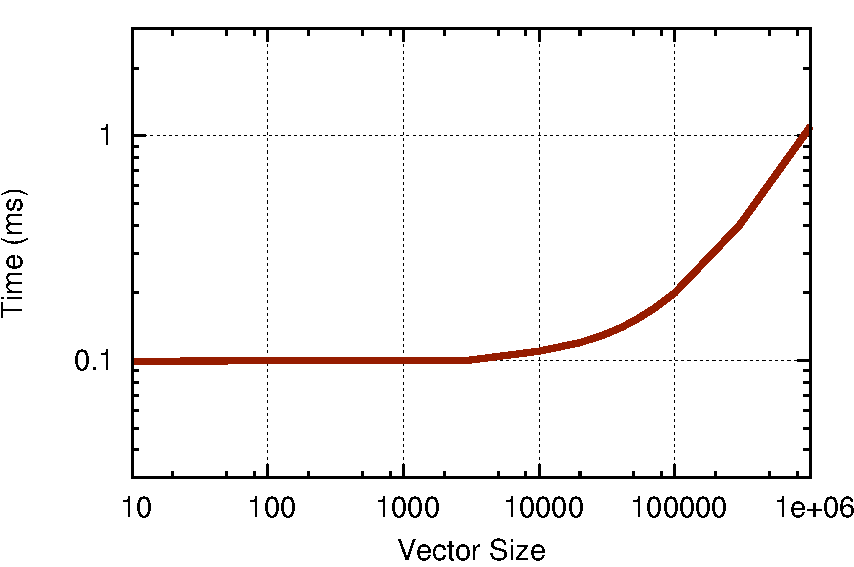
\includegraphics[width=0.6\textwidth]{figs/kernel-launch.pdf} \end{center}
 \end{block}

 \begin{block}{OpenCL Kernel Launch Overhead}
   \begin{itemize}
    \item $10-100$ $\mu$s
   \end{itemize}
 \end{block}

\end{frame}



\begin{frame}[fragile]
\frametitle{Performance}
 \begin{block}{GPUs: Disillusion - Computing Architecture Schematic}
  \begin{center}
   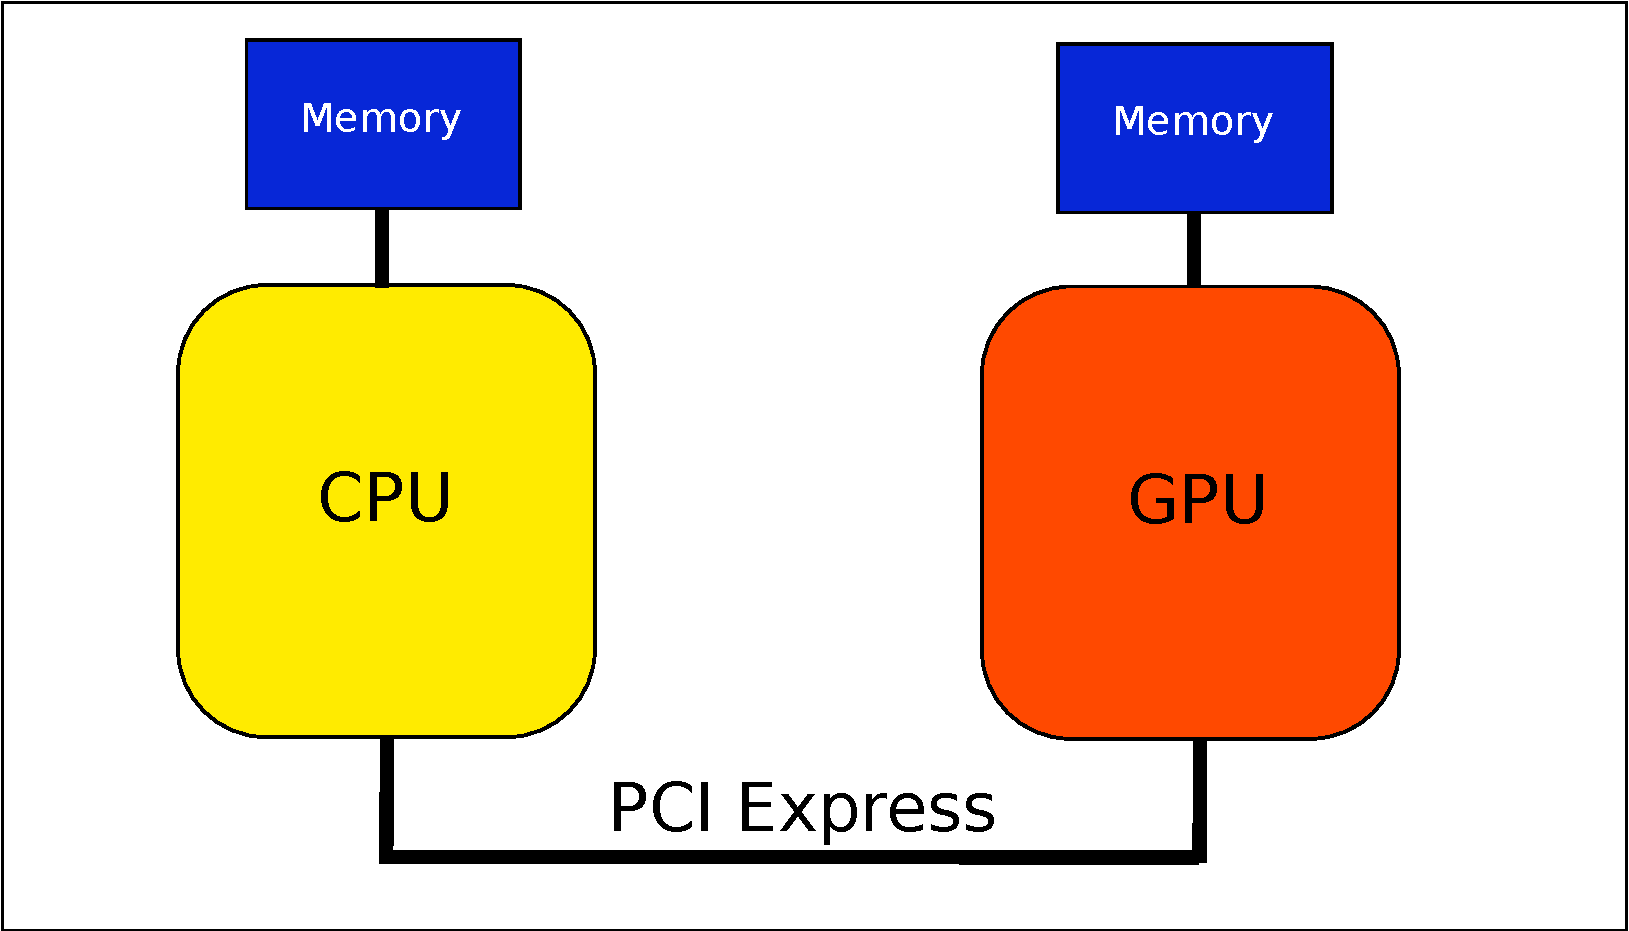
\includegraphics[width=0.7\textwidth]{figs/cpu-gpu-coarse.pdf}
  \end{center}

 
 \begin{itemize}
  \item \vspace*{1.12cm}
 \end{itemize}
 \end{block}

\end{frame}

\begin{frame}[fragile]
\frametitle{Performance}
 \begin{block}{GPUs: Disillusion - Computing Architecture Schematic}
  \begin{center}
   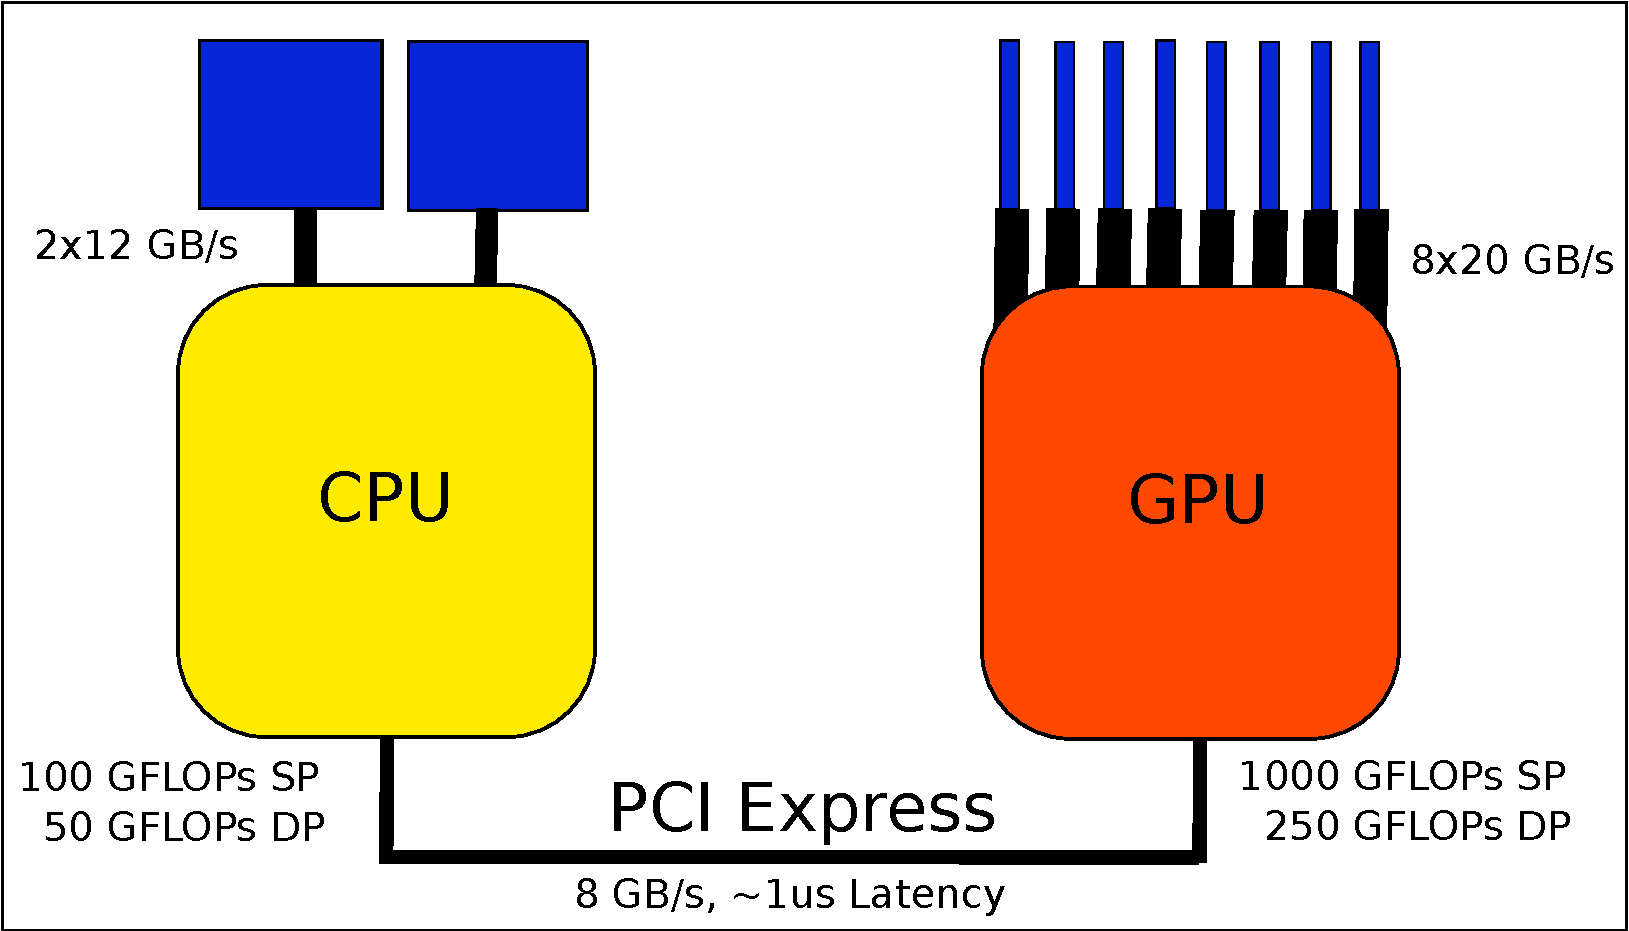
\includegraphics[width=0.7\textwidth]{figs/cpu-gpu-detail.pdf}
  \end{center}

 \begin{itemize}
  \item Good for large FLOP-intensive tasks, high memory bandwidth
  \item PCI-Express can be a bottleneck
  \item $\gg 10$-fold speedups (usually) not backed by hardware
 \end{itemize}
 \end{block}

\end{frame}



\begin{frame}{Performance}
\begin{block}{Some benchmarks - vector addition}
  \begin{center}
   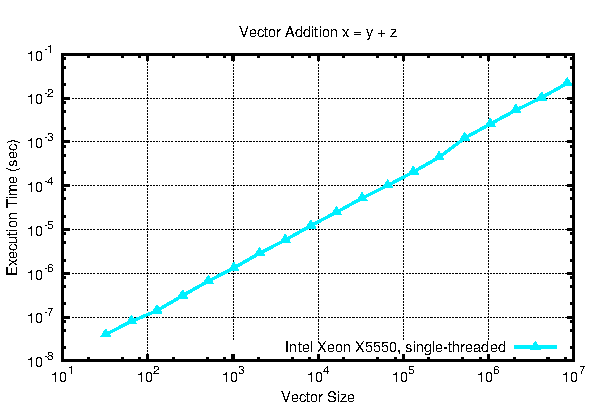
\includegraphics[width=0.9\textwidth]{figs/vector-timings-1}
  \end{center}
\end{block}
\end{frame}

\begin{frame}{Performance}
\begin{block}{Some benchmarks - vector addition}
  \begin{center}
   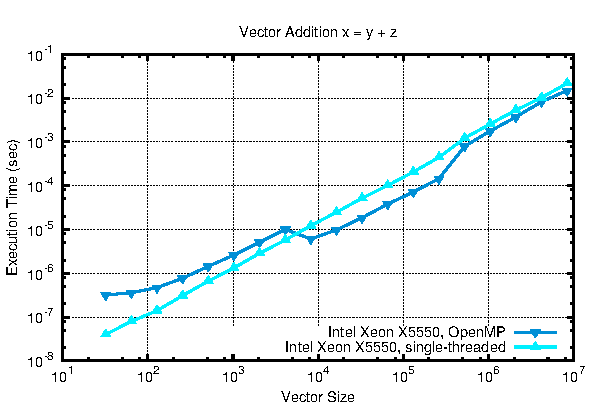
\includegraphics[width=0.9\textwidth]{figs/vector-timings-2}
  \end{center}
\end{block}
\end{frame}

\begin{frame}{Performance}
\begin{block}{Some benchmarks - vector addition}
  \begin{center}
   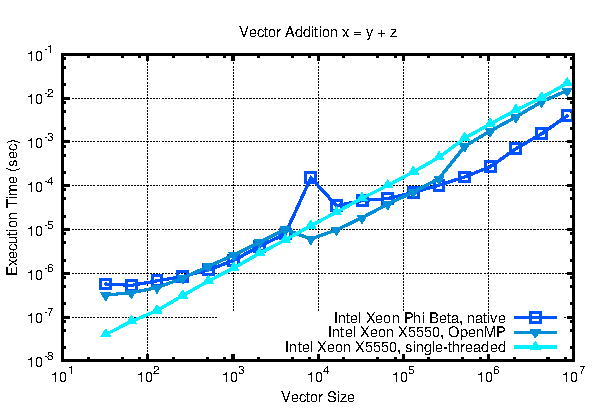
\includegraphics[width=0.9\textwidth]{figs/vector-timings-3}
  \end{center}
\end{block}
\end{frame}

\begin{frame}{Performance}
\begin{block}{Some benchmarks - vector addition}
  \begin{center}
   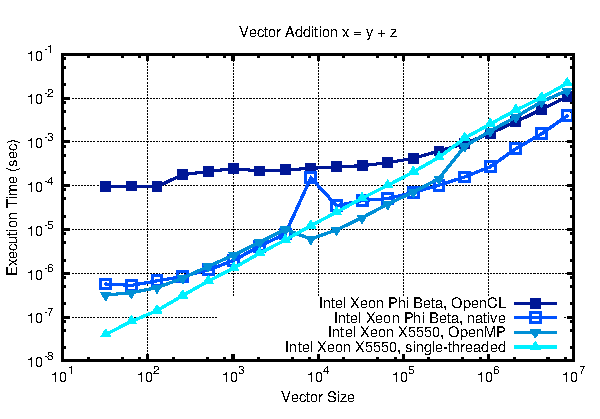
\includegraphics[width=0.9\textwidth]{figs/vector-timings-4}
  \end{center}
\end{block}
\end{frame}

\begin{frame}{Performance}
\begin{block}{Some benchmarks - vector addition}
  \begin{center}
   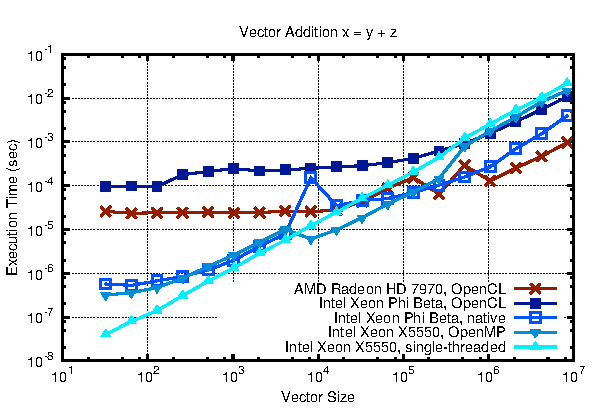
\includegraphics[width=0.9\textwidth]{figs/vector-timings-5}
  \end{center}
\end{block}
\end{frame}

\begin{frame}{Performance}
\begin{block}{Some benchmarks - vector addition}
  \begin{center}
   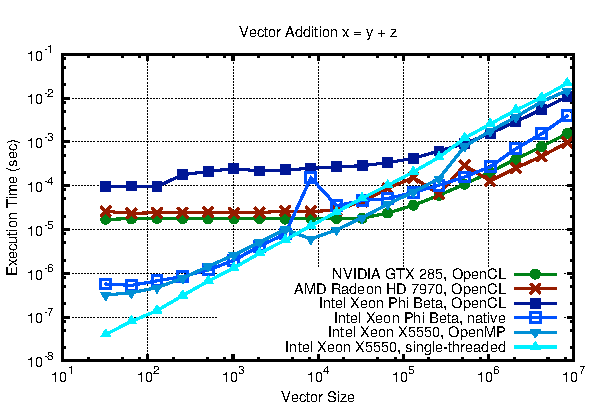
\includegraphics[width=0.9\textwidth]{figs/vector-timings-6}
  \end{center}
\end{block}
\end{frame}

\begin{frame}{Performance}
\begin{block}{Some benchmarks - vector addition}
  \begin{center}
   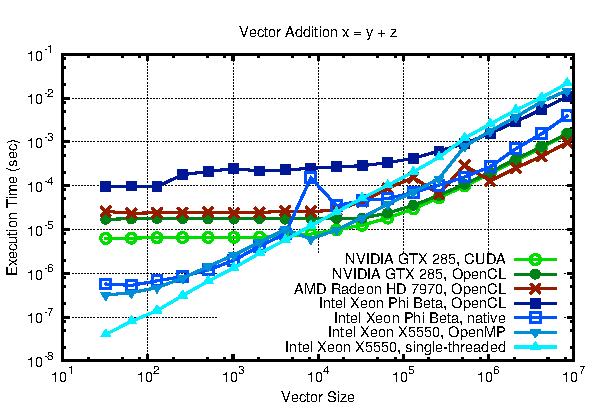
\includegraphics[width=0.9\textwidth]{figs/vector-timings-7}
  \end{center}
\end{block}
\end{frame}



\begin{frame}{Performance}
\begin{block}{Some benchmarks - CG solver}
  \begin{center}
   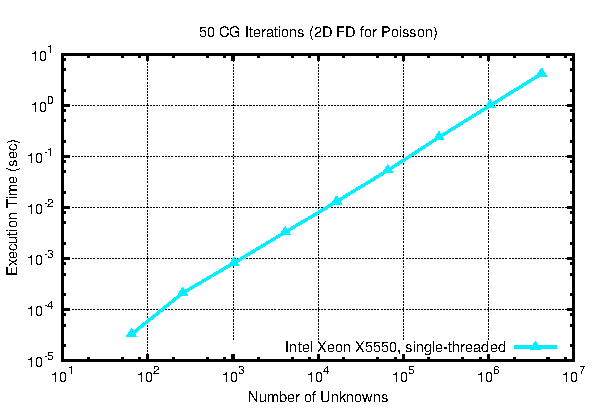
\includegraphics[width=0.9\textwidth]{figs/cg-timings-1}
  \end{center}
\end{block}
\end{frame}

\begin{frame}{Performance}
\begin{block}{Some benchmarks - CG solver}
  \begin{center}
   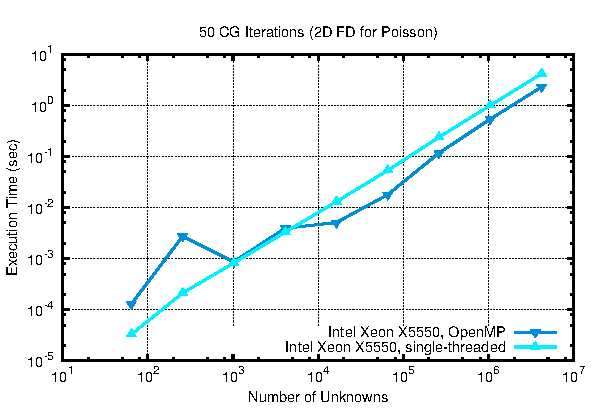
\includegraphics[width=0.9\textwidth]{figs/cg-timings-2}
  \end{center}
\end{block}
\end{frame}

\begin{frame}{Performance}
\begin{block}{Some benchmarks - CG solver}
  \begin{center}
   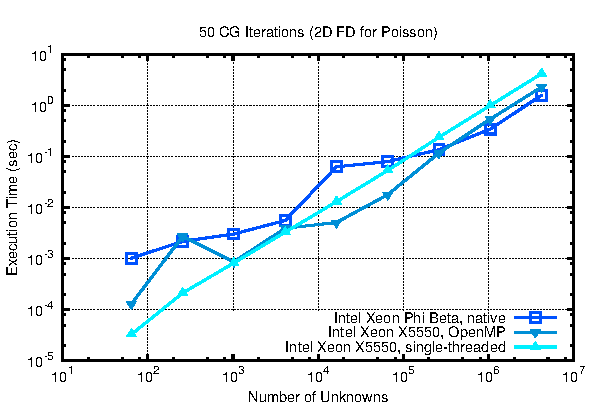
\includegraphics[width=0.9\textwidth]{figs/cg-timings-3}
  \end{center}
\end{block}
\end{frame}

\begin{frame}{Performance}
\begin{block}{Some benchmarks - CG solver}
  \begin{center}
   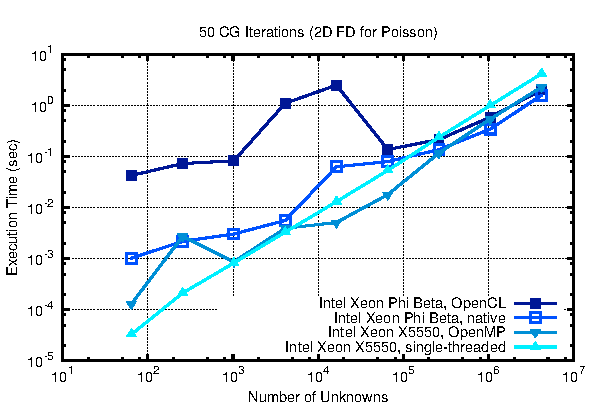
\includegraphics[width=0.9\textwidth]{figs/cg-timings-4}
  \end{center}
\end{block}
\end{frame}

\begin{frame}{Performance}
\begin{block}{Some benchmarks - CG solver}
  \begin{center}
   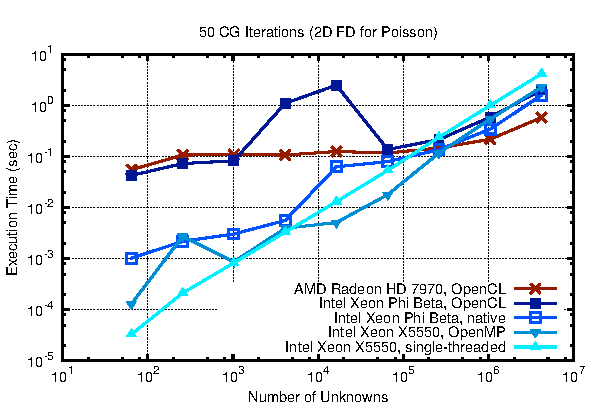
\includegraphics[width=0.9\textwidth]{figs/cg-timings-5}
  \end{center}
\end{block}
\end{frame}

\begin{frame}{Performance}
\begin{block}{Some benchmarks - CG solver}
  \begin{center}
   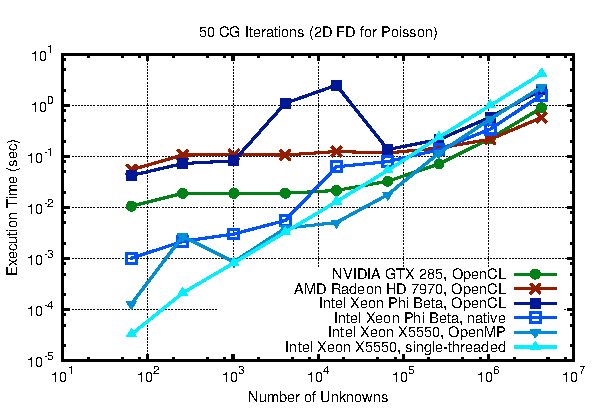
\includegraphics[width=0.9\textwidth]{figs/cg-timings-6}
  \end{center}
\end{block}
\end{frame}

\begin{frame}{Performance}
\begin{block}{Some benchmarks - CG solver}
  \begin{center}
   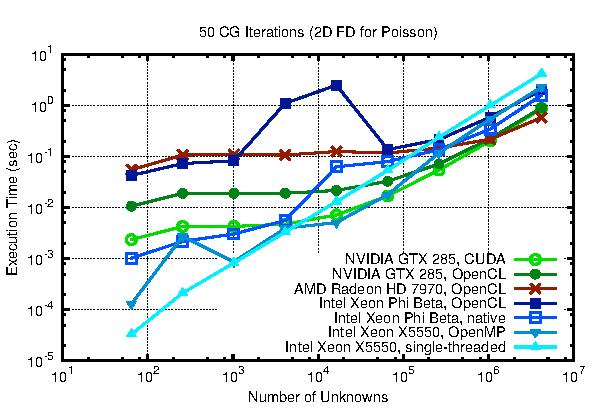
\includegraphics[width=0.9\textwidth]{figs/cg-timings-7}
  \end{center}
\end{block}
\end{frame}



\begin{frame}{Performance}
 \begin{block}{Some benchmarks - Matrix-Matrix Multiplication}
  \begin{itemize}
   \item Auto-tuning environment  (AMD Radeon HD 7970, single precision)
   \item 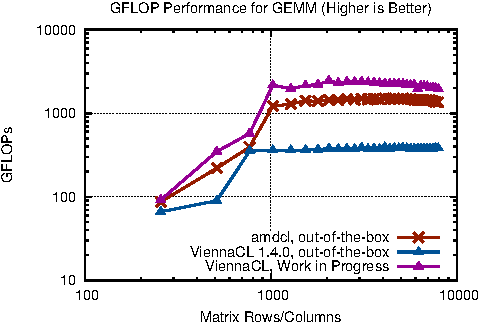
\includegraphics[width=0.85\textwidth]{figs/gemm3.pdf}
  \end{itemize}
 \end{block}
\end{frame}





\begin{frame}{Summary}
\begin{block}{What have we learned?}
  \begin{itemize}
   \item What are subvectors/submatrices and how to use them
   \item How to eliminate temporaries
   \item Expression templates and when they help us
   \item Interface to Eigen
   \item ViennaCL isn't optimized for small vectors/matrices
   \item Performance bottleneck
   \item Overview of ViennaCL performance
  \end{itemize}
\end{block}
\end{frame}


% \begin{frame}{Summary}
% \TODO{Achievement unlocked: ViennaCL expert}
% \end{frame}
















